%%%%%%%%%%%%%%%%%%%%%%%%%%%%%%%%%%%%%%%%%%%%%%%%%%%%%%%%%%%%
% Paul McKee
% Rensselaer Polytechnic Institute
% 1/31/18
% Master's Thesis
% with Dr. Kurt Anderson
% LaTeX Template: Project Titlepage Modified (v 0.1) by rcx
%%%%%%%%%%%%%%%%%%%%%%%%%%%%%%%%%%%%%%%%%%%%%%%%%%%%%%%%%%%%

\documentclass[12pt]{article}
\iffalse


\usepackage[a4paper]{geometry}
\usepackage[utf8]{inputenc}
\usepackage[myheadings]{fullpage}
\usepackage{fancyhdr}
\usepackage{lastpage}
\usepackage{graphicx, wrapfig, subcaption, setspace, booktabs}
\usepackage[T1]{fontenc}
\usepackage[font=small, labelfont=bf]{caption}
\usepackage{fourier}
\usepackage[protrusion=true, expansion=true]{microtype}
\usepackage[english]{babel}
\usepackage{sectsty}
\usepackage{url, lipsum}
\usepackage{makecell}
\usepackage{amsmath}
\usepackage{setspace}
\usepackage{amsmath}
\usepackage{titlesec}
\usepackage[table,xcdraw]{xcolor}
%\titleformat{\section}{\normalfont\fontsize{25}{25}\bfseries}{\thesection}{1em}{}

%\usepackage[format=hang,font={small,bf},labelfont=bf]{caption}

\usepackage{listings}
\usepackage{color} %red, green, blue, yellow, cyan, magenta, black, white
\definecolor{mygreen}{RGB}{28,172,0} % color values Red, Green, Blue
\definecolor{mylilas}{RGB}{170,55,241}

%\newcommand{\HRule}[1]{\rule{\linewidth}{#1}}
\setcounter{tocdepth}{5}
\setcounter{secnumdepth}{5}
\usepackage{fancyhdr}
\usepackage{lastpage}
\usepackage{graphicx}
%\pagestyle{fancy}
%\fancyhf{Philip Hoddinott, Module 4 Questions}
\fancyhf{}
%\fancyhead[L]{Philip Hoddinott}
%\fancyhead[C]{Project 2}
%\fancyhead[R]{\leftmark}

\fancyhead[L]{Master's Thesis}
%\fancyhead[C]{\thepage}
%\fancyhead[R]{Module 5 Homework}
\fancyhead[C]{\rightmark}
\fancyhead[R]{Philip Hoddinott}
\fancypagestyle{plain}{
	\fancyfoot[C]{\thepage}}
\usepackage{float}

%\rfoot{Page \thepage \hspace{1pt} of \pageref{LastPage}}

\newcommand{\N}{\mathbb{N}}
\newcommand{\Z}{\mathbb{Z}}
\renewcommand{\headrulewidth}{0pt} % remove the header rule
\rfoot{\thepage}



\fi


\usepackage{blindtext}
\usepackage[utf8]{inputenc}

\usepackage{graphicx, wrapfig, subcaption, setspace, booktabs}
\usepackage{sectsty}
\usepackage{url, lipsum}
\usepackage{makecell}
\usepackage{amsmath}
\usepackage{setspace}
\usepackage{amsmath}
\usepackage{color} %red, green, blue, yellow, cyan, magenta, black, white
\definecolor{mygreen}{RGB}{28,172,0} % color values Red, Green, Blue
\definecolor{mylilas}{RGB}{170,55,241}

\usepackage[table,xcdraw]{xcolor}


\usepackage[margin=1in]{geometry} 
\usepackage{amsmath,amsthm,amssymb}
\usepackage{color}
\usepackage{fancyhdr}
\usepackage{lastpage}
\usepackage{graphicx}
%\usepackage{blindtext}
%\usepackage{titleps,kantlipsum}
%\let\Sectionmark\sectionmark
%\def\sectionmark#1{\def\Sectionname{#1}\Sectionmark{#1}}
%\let\Subsectionmark\subsectionmark
%\def\subsectionmark#1{\def\Subsectionname{#1}\Subsectionmark{#1}}
%\let\Subsubsectionmark\subsubsectionmark
%\def\subsubsectionmark#1{\def\Subsubsectionname{#1}\Subsubsectionmark{#1}}

\pagestyle{fancy}
\fancyhf{}
%\fancyhead[L]{Master's Thesis}
%\fancyhead[C]{\rightmark}


%\fancyhead[C]{\nouppercase{\leftmark}}
\fancyhead[L]{\nouppercase{\leftmark}}
\fancyhead[R]{Philip Hoddinott}
%\fancyhead[C]{\thesubsection.\ \Subsectionname}
%\fancyhead[C]{\subsectiontitle}
\rfoot{Page \thepage \hspace{1pt} of \pageref{LastPage}}

\newcommand{\N}{\mathbb{N}}
\newcommand{\Z}{\mathbb{Z}}

\newenvironment{theorem}[2][Theorem]{\begin{trivlist}
		\item[\hskip \labelsep {\bfseries #1}\hskip \labelsep {\bfseries #2.}]}{\end{trivlist}}
\newenvironment{lemma}[2][Lemma]{\begin{trivlist}
		\item[\hskip \labelsep {\bfseries #1}\hskip \labelsep {\bfseries #2.}]}{\end{trivlist}}
\newenvironment{exercise}[2][Exercise]{\begin{trivlist}
		\item[\hskip \labelsep {\bfseries #1}\hskip \labelsep {\bfseries #2.}]}{\end{trivlist}}
\newenvironment{problem}[2][Problem]{\begin{trivlist}
		\item[\hskip \labelsep {\bfseries #1}\hskip \labelsep {\bfseries #2.}]}{\end{trivlist}}
\newenvironment{question}[2][Question]{\begin{trivlist}
		\item[\hskip \labelsep {\bfseries #1}\hskip \labelsep {\bfseries #2.}]}{\end{trivlist}}
\newenvironment{corollary}[2][Corollary]{\begin{trivlist}
		\item[\hskip \labelsep {\bfseries #1}\hskip \labelsep {\bfseries #2.}]}{\end{trivlist}}

\newenvironment{solution}{\begin{proof}[Solution]}{\end{proof}}
\usepackage{multicol}
\newcommand{\mysize}{0.5}
\usepackage{subcaption}
\usepackage{float}
\usepackage{listings}
\usepackage{color} 
\newcolumntype{L}{>{\centering\arraybackslash}m{3cm}}
\usepackage{setspace}
\usepackage[framed,numbered,autolinebreaks,useliterate]{mcode}
\renewcommand{\captionfont}{\bfseries}



% %---------------------------------------------------------------
% % HEADER & FOOTER
% %---------------------------------------------------------------

%\fancyhf{}
%\pagestyle{fancy}
%\renewcommand{\headrulewidth}{0pt}
%\setlength\headheight{0pt}
%\fancyhead[L]{ Paul McKee }
%\fancyhead[R]{Rensselaer Polytechnic Institute}
%\cfoot{ \thepage\ } 


%--------------------------------------------------------------
% TITLE PAGE
%--------------------------------------------------------------

\begin{titlepage}
	\title{ 
		\LARGE \textbf{\uppercase{Tracking of space debris from publicly available data }} \\
		\vspace{0.25cm}
		\LARGE \textbf{Philip Hoddinott}
	}
	\author{\small{Submitted in Partial Fulfillment of the Requirements} \\ \small{for the Degree of} \\
		\uppercase{Master of Science} \\ \\
		Approved by:
		\\ Kurt Anderson, Chair \\ John Christian \\ Matthew Oehlschlaeger \\ \\ %% from paul's template
		
\includegraphics[width=2.5cm]{rensselaer_seal.png} \\
		\small{\textit{Department of Mechanical, Aerospace, and Nuclear Engineering}} \\
		\small{Rensselaer Polytechnic Institute} \\ 
		\small{Troy, New York} \\
		\small{November 2018}
	}
\end{titlepage}

\begin{document}
	\maketitle
	
	
	\pagenumbering{roman}
	\setcounter{page}{-1}
	% --Table of Contents----------

	\newlength\longest
	\clearpage
	
	\thispagestyle{empty}
	\null\vfill
	
	\begin{figure}[!t]
		\begin{center}
			\settowidth\longest{\huge\itshape But, Captain, I cannot change;}
			\parbox{\longest}{%
				\raggedright{\huge\itshape%
					But, Captain, I cannot change the laws of physics\par\bigskip
				}   
				\raggedleft\Large{-Lt. Commander Montgomery ``Scotty" Scott}\par
				\raggedleft\Large{USS}\textit{ Enterprise}\par%
				
			}
		\end{center}
	\end{figure}

	
	\null\vfill
	
	%		\begin{figure}
	%	\centering
	%	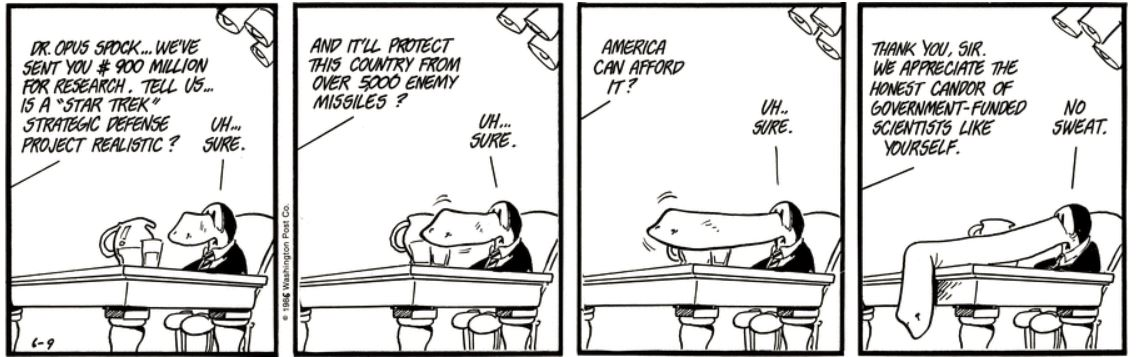
\includegraphics[width=0.7\linewidth]{../../Bloom_County_2}
	%	\caption*{}
	%	\label{fig:bloomcounty2}
	%\end{figure}
	
	\begin{figure}
		\centering
		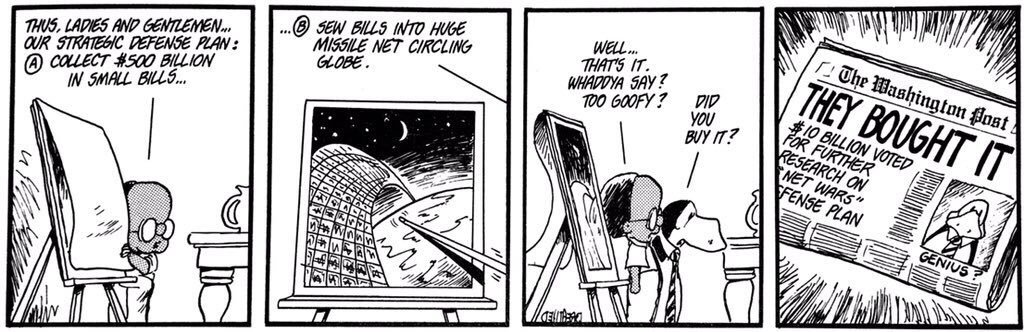
\includegraphics[width=0.7\linewidth]{../../Bloom_County}
		\caption*{}
		\label{fig:bloomcounty}
	\end{figure}
	
	\newpage
	%	\newpage
	\tableofcontents
	\newpage

	%\thispagestyle{fancy}
	
	%\addcontentsline{toc}{section}{\uppercase{Table of Contents}}
	\listoftables
	%\addcontentsline{toc}{section}{\uppercase{List of Tables}}
	\listoffigures
	%\addcontentsline{toc}{section}{\uppercase{List of Figures}}
	% -----------------------------
	
	% ------------------------------------------------------------
	% Acknowledgement
	% ------------------------------------------------------------
	\newpage
		\doublespacing
	\section{Acknowledgments}
	%\addcontentsline{toc}{section}{\uppercase{Acknowledgement}}
	

	This paper would never have been possible with out the help of so many people. I am indebted to my parents and my brother for their support. My teachers and professors who have helped me along the way have my deepest gratitude. I am thankful towards Paul McKee for his assistance with Latex and to John Benke for his assistance with Github and PHP. I am incredibly thankful towards my Advisor Professor Kurt Anderson for his support and his many phenomenal stories. Issac Newton once said ``If I have seen further it is by standing on the shoulders of giants"\cite{newtLettr}. I would like to thank you all for being my giants.
	
	
	
	

	
	% ------------------------------------------------------------
	% Abstract 
	% ------------------------------------------------------------
	
	\newpage
	\section{Abstract}
	The purpose of this thesis is to develop software that will acquire information about earth orbiting debris, turn the information into a usable format for someone with basic orbital mechanics experience. The code will take in parameters about the orbital data from the user. Then it checks for existing files and communicates with NORAD servers. The data is downloaded from NORAD and converted from the Two Line Element set format to Keplerian Orbital Elements. From here the data may be sorted according to the user's desire. The code will be able to handle errors that occur during the process.
	\iffalse
	 \textcolor{red}{and develop a targeting algorithm for a debris removal satellite}. The information is things such as orbital elements, debris size, \textcolor{red}{ and sping if i can find htis.} \par 
	 Should this be accomplished in a timely manner more work will be done on the orbital dynamics of OSCAR getting to said debris.
	 \fi
	% ------------------------------------------------------------
	% Introduction
	% ------------------------------------------------------------
	\newpage
	\pagenumbering{arabic} % this should start the normal numberinbg
	\section{Introduction}
	Before the methods of this project are explored, the background of the problem must first be presented. Space debris and the threat they pose will be explained, as well as the proposed solution. 
	

	\subsection{Space Debris}
	
	March 17th, 1958 the Vanguard 1 satellite was launched. It was the fourth man made satellite. Despite communication being lost in the 1960s, it is still in orbit to this day. \par 
	
	\begin{figure}[h!]
		\centering
		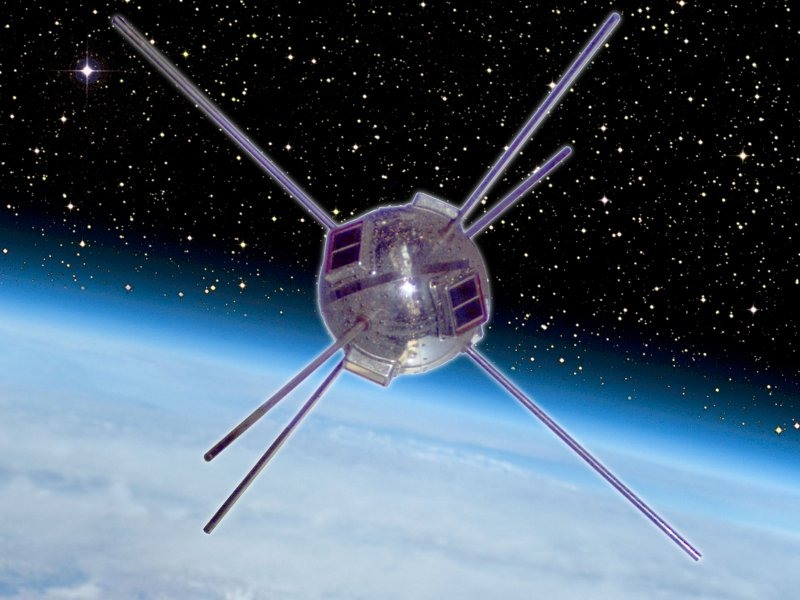
\includegraphics[width=0.7\linewidth]{Vanguard_1_composite}
		\caption{Artist's rendition of Vanguard 1 in orbit\cite{usnrl_2008}.}
		\label{fig:vanguard1composite}
	\end{figure}
	
	While spacecraft are supposed to be moved to a graveyard orbit, not all are. These large objects would be catastrophic if they collided with another object in orbit. However large objects do not pose the greatest threat. Their size makes them easy to track and there are comparatively little of them. 
	
	\begin{figure}
		\centering
		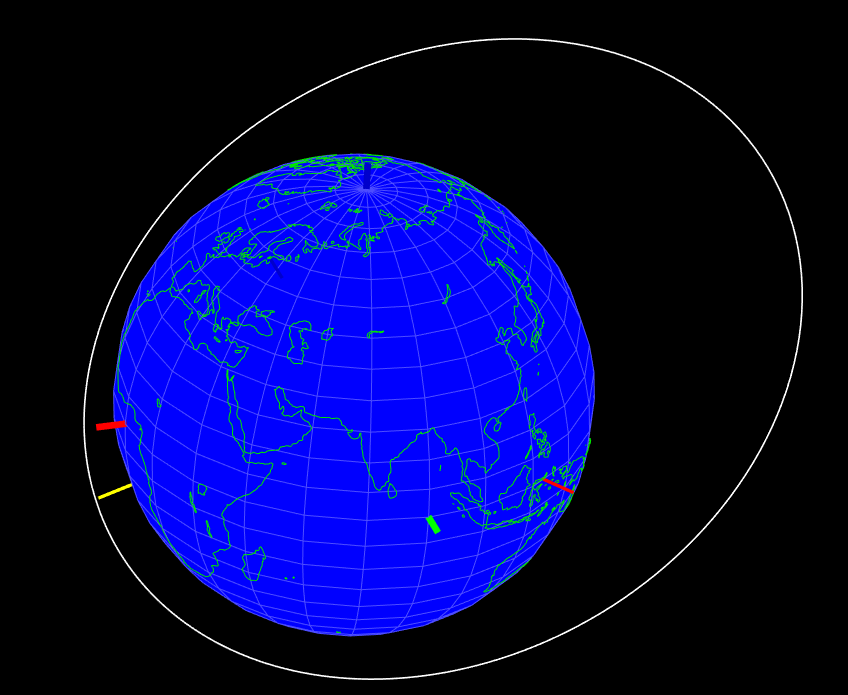
\includegraphics[width=0.7\linewidth]{Vanguard_1_orbit}
		\caption{Vanguard's Orbit as of 10/17/2018}
		\label{fig:vanguard1orbit}
	\end{figure}

	The debris that poses the greatest threat are the smaller pieces. Their size makes them harder to track and predict trajectories. And they are numerous. As of 2013 it is estimated that there are:\par 

	
	\begin{itemize}\singlespacing
		\item 	29,000 Objects larger than 10 cm.
		\item 	670,000 Objects larger than 1 cm.
		\item 	Over 170,000,000 Objects larger than 1 mm.
	\end{itemize}	\doublespacing
	
	These objects can do grievous harm to people or objects in space. A 10 cm object can cause the destruction of a satellite, a 1 cm object could penetrate the ISS's shields putting lives at risk and a 1 mm object could destroy critical subsystems.\cite{sdor2014} The impact of one of these objects is shown in figure \ref{fig:sts7crack}.
	
	
	
	\begin{figure}
		\centering
		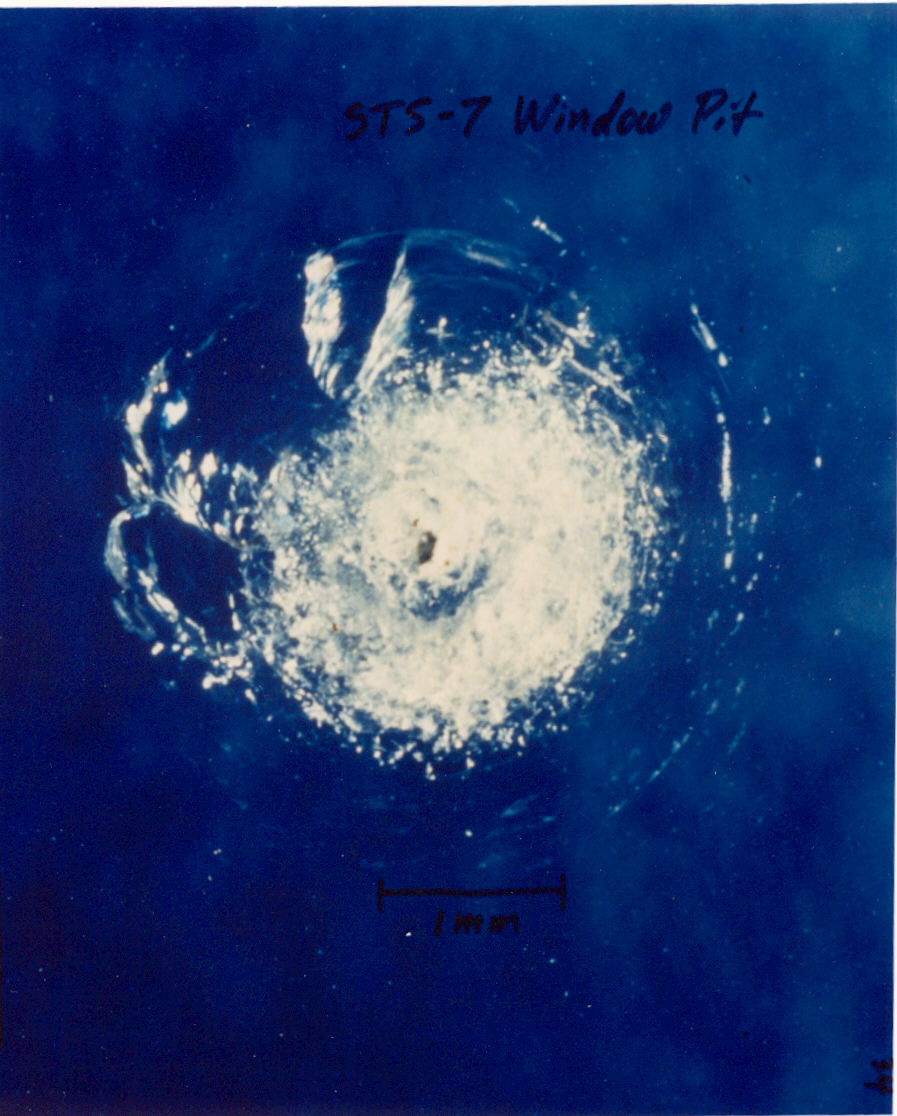
\includegraphics[width=0.7\linewidth]{sts7crack}
		\caption{An impact crater on one of the windows of the Space Shuttle Challenger following a collision with a micrometeoroid\cite{stscrack}}
		\label{fig:sts7crack}
	\end{figure}


\begin{figure}
	\centering
	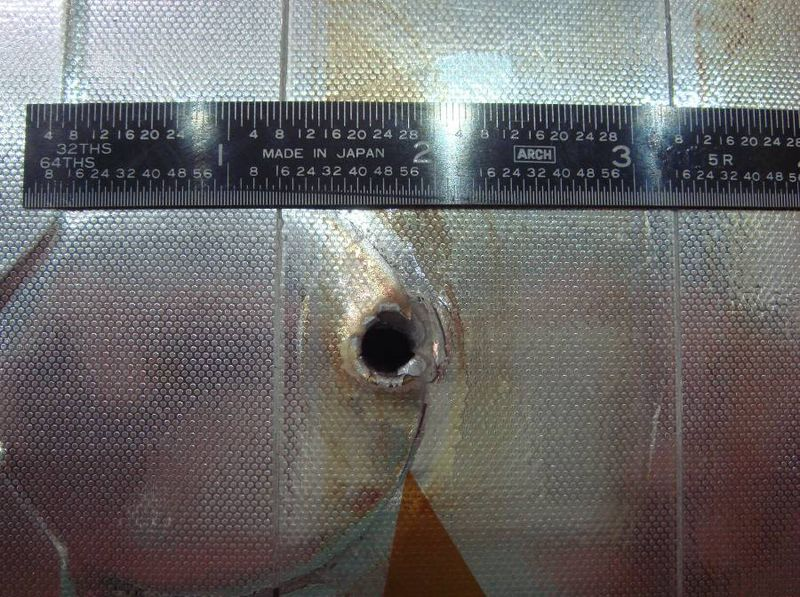
\includegraphics[width=0.7\linewidth]{STS-118_debris_entry}
	\caption{Debris impact on Space Shuttle Endeavorer's radiator panel\cite{endevHole}}
	\label{fig:sts-118debrisentry}
\end{figure}
	
	
	%\begin{align}
	%E=\frac{1}{2}mv^2
	%\end{align}
	%\begin{align}
	%E=\frac{1}{2}(.001kg)(7.66 \times 10^3)^2
	%\end{align}
	
	\subsection{Kessler Syndrome}
	More than just harm to individual spacecraft or persons there is the threat of Kessler Syndrome. Also known as the Kessler effect or collision cascading, this is a scenario where there are enough objects in low earth orbit that a collision between objects will cause a chain reaction creating more and more space debris. This could result in space being inaccessible for years to come, as any object that left the earth's atmosphere would be immediately shredded by debris (thus adding even more debris).\par 
	
	This can be prevented by moving derelict spacecraft to graveyard orbits. However even spacecraft in graveyard orbits are not perfectly safe. Coolant tanks can puncture and coolant droplets freeze adding to the debris. \par 
	
	The alternative is to lower the orbit until it experiences atmospheric effects. But if the debris's orbit keeps it out of the atmosphere, then the debris must be moved. 

	\subsection{CubeSats}
	For the task of moving debris, a CubeSat will be used. CubeSats are a type of miniaturized satellite. CubeSats get their name from their structure, they are made up of one or more $10\times10\times10$ cm units.	These units have a maximum mass of 1.33 kilograms. First launched in 1998, as of August 2018, there have been 875 CubeSats launched\cite{nanosats_eu}. \par 
	
	
	
	CubeSats are used for projects that are too risky for a larger more expensive satellite, often demonstrating new technologies. They can take on larger risks due to their low cost. As such CubeSats are common for experiential missions such as this one.
	
	\subsection{OSCAR}
	There is a CubeSat currently being designed by Rensselaer Polytechnic Institute (RPI). This CubeSat's goal is to deorbit space debris by use of a magnetic tether. \par 
	
	
	This CubeSat is called O.S.C.A.R, which is short for “Obsolete Satellite Capture and Recovery”. It should be noted that this name is only temporary and will likely change in the near future. However for the purposes of this report, the RPI CubeSat will be referred to as OSCAR.\par 
	
	OSCAR will be a three unit  $(10\times10\times30)$ CubeSat with a mass of four kilograms. It will be able to remove four pieces of space debris.\cite{paulT} For OSCAR to be able to deorbit space debris, it must know where the space debris is. 
	
	\subsection{Orbital Elements}
	
	This thesis is concerned with the acquisition of current orbital data of space debris and it's transformation into useful formats. 
	
	First orbital elements should be defined. Orbital elements are the parameters that define an orbit. The traditional Keplerian elements found in many textbooks are as follows: 
	
	\singlespacing
	
	\begin{eqnarray}
	h& \text{specific angular momentum}\nonumber\\
	i& \text{ inclination}\nonumber\\
	\Omega &\text{ right ascension (RA) of the ascending node}\nonumber\\
	e & \text{ eccentricity}\nonumber\\
	\omega &\text{ argument of perigee}\nonumber\\
	\theta &\text{ True anomaly}
	\end{eqnarray}
	
	They may be seen in figure \ref{fig:curtisoe}.
	
	\begin{figure}[H]
		\centering
		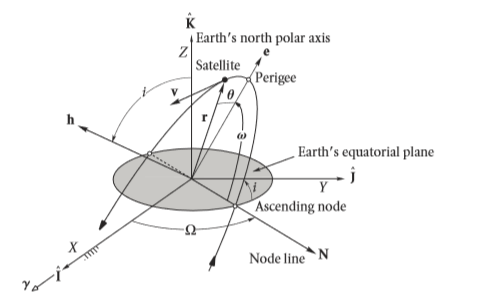
\includegraphics[width=0.7\linewidth]{curtis_OE}
		\caption{Geocentric equatorial frame and the orbital elements\cite{curtis2013}.}
		\label{fig:curtisoe}
	\end{figure}
	
	\doublespacing
	However for space debris the following set of orbital elements is slightly more useful. \par 
	
	\singlespacing
	
	\begin{eqnarray}
	e & \text{ eccentricity}\nonumber\\
	a & \text{ semimajor axis}\nonumber\\
	i& \text{ inclination}\nonumber\\
	\Omega &\text{ right ascension (RA) of the ascending node}\nonumber\\
	\omega &\text{ argument of perigee}\nonumber\\
	\nu &\text{ Mean anomaly}
	\end{eqnarray}
	
	\doublespacing
	
	This is preferable as the semi major axis is used in conjunction with eccentricity with it's relation to perigee and apogee.  However this is not a hard rule, and the code could be altered to use the first set of orbital elements. The orbital elements are better demonstrated in figure \ref{fig:nasaoe1} and figure \ref{fig:nasaoe2}
	
	\begin{figure}
		\centering
		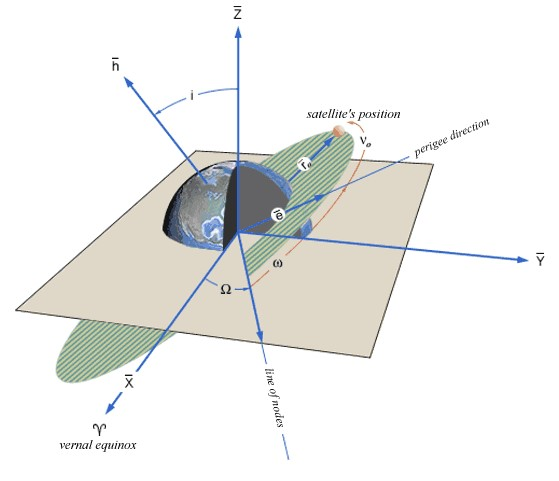
\includegraphics[width=0.7\linewidth]{nasaOE1}
		\caption{Diagram of Earth and Orbital Elements as well as Cartesian State Vectors\cite{nasaOE}}
		\label{fig:nasaoe1}
	\end{figure}
	\begin{figure}
		\centering
		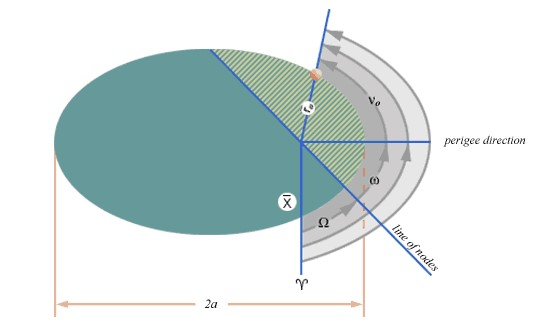
\includegraphics[width=0.7\linewidth]{nasaOE2}
		\caption{Diagram of Earth and Orbital Elements\cite{nasaOE}}
		\label{fig:nasaoe2}
	\end{figure}
	
	


% Please add the following required packages to your document preamble:
% \usepackage[table,xcdraw]{xcolor}
% If you use beamer only pass "xcolor=table" option, i.e. \documentclass[xcolor=table]{beamer}
\begin{table}[]
	\caption{Orbital Elements and their symbols\cite{nasaOE}}
	\label{tab:NASA_Orbt_elem}
	
	\begin{tabular}{|p{3.75cm}|l|p{10.25cm}|}
		\hline
		Name & Symbol & Description               \\ \hline
		Semi-major axis & a & Defines the size of the orbit. \\ \hline
		Eccentricity & e & Defines the shape of the orbit. \\ \hline
		Inclination & i & Defines the orientation of the orbit with respect to the Earth's equator. \\ \hline
		Argument of Perigee & $\omega$  & Defines where the low point, perigee, of the orbit is with respect to the Earth's surface. \\ \hline
		Right Ascension of the Ascending Node & $\Omega$  & Defines the location of the ascending and descending orbit locations with respect to the Earth's equatorial plane. \\ \hline
		True/Mean Anomaly & $\nu$  & Defines where the satellite is within the orbit with respect to perigee. \\ \hline
			
		\iffalse
		
		{
			>{\columncolor[HTML]{EEEEEE}}l 
			>{\columncolor[HTML]{EEEEEE}}l 
			>{\columncolor[HTML]{EEEEEE}}l }
		\multicolumn{3}{c}{\cellcolor[HTML]{6699CC}{\color[HTML]{FFFFFF} \textbf{Orbital Elements:}}}
		                                                                  \\
		                                                                  	%\begin{tabular}{|p{4cm}|p{11.5cm}|}
Name & Symbol & Description               \\ \hline
		Semi-major axis                       & a & Defines the size of the orbit.                                                                                     \\
		Eccentricity                          & e & Defines the shape of the orbit.                                                                                    \\
		Inclination                           & i & \multicolumn{1}{m{8cm}}{\cellcolor[HTML]{EEEEEE}Defines the orientation of the orbit with respect to the Earth's equator.}                              \\
		Argument of Perigee                   &$\omega$   & \multicolumn{1}{m{8cm}}{\cellcolor[HTML]{EEEEEE}Defines where the low point, perigee, of the orbit is with respect to the Earth's surface.}                         \\
		Right Ascension of the Ascending Node &$\Omega$   & \multicolumn{1}{m{8cm}}{\cellcolor[HTML]{EEEEEE}Defines the location of the ascending and descending orbit locations with respect to the Earth's equatorial plane.} \\
		True/Mean Anomaly                     & $\nu$  & \multicolumn{1}{m{8cm}}{\cellcolor[HTML]{EEEEEE}Defines where the satellite is within the orbit with respect to perigee.}     
		\fi                                     
	\end{tabular}
\end{table}


	
\iffalse

% Please add the following required packages to your document preamble:
% \usepackage[table,xcdraw]{xcolor}
% If you use beamer only pass "xcolor=table" option, i.e. \documentclass[xcolor=table]{beamer}
\begin{table}[]
	\caption{Orbital Elements and their symbols\cite{nasaOE}}
	\label{my-label}
	\begin{tabular}{
			>{\columncolor[HTML]{EEEEEE}}l 
			>{\columncolor[HTML]{EEEEEE}}l 
			>{\columncolor[HTML]{EEEEEE}}l }
		\multicolumn{3}{c}{\cellcolor[HTML]{6699CC}{\color[HTML]{FFFFFF} \textbf{Orbital Elements:}}}                                                                  \\
		Semi-major axis                       & a & Defines the size of the orbit.                                                                                     \\
		Eccentricity                          & e & Defines the shape of the orbit.                                                                                    \\
		Inclination                           & i & \multicolumn{1}{m{8cm}}{\cellcolor[HTML]{EEEEEE}Defines the orientation of the orbit with respect to the Earth's equator.}                              \\
		Argument of Perigee                   &$\omega$   & \multicolumn{1}{m{8cm}}{\cellcolor[HTML]{EEEEEE}Defines where the low point, perigee, of the orbit is with respect to the Earth's surface.}                         \\
		Right Ascension of the Ascending Node &$\Omega$   & \multicolumn{1}{m{8cm}}{\cellcolor[HTML]{EEEEEE}Defines the location of the ascending and descending orbit locations with respect to the Earth's equatorial plane.} \\
		True/Mean Anomaly                     & $\nu$  & \multicolumn{1}{m{8cm}}{\cellcolor[HTML]{EEEEEE}Defines where the satellite is within the orbit with respect to perigee.}                                          
	\end{tabular}
\end{table}
\fi
	
\iffalse
	\begin{itemize}
		\item eccentricity (e)
		
		The eccentricity is the shape of the ellipse. An eccentricity of 1 is a circle.
		\item Semi-major axis (a)
		\begin{figure}
			\centering
			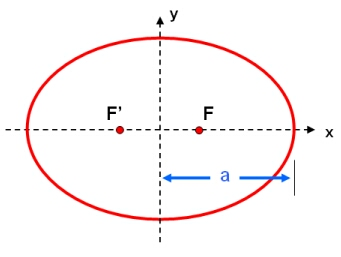
\includegraphics[width=0.7\linewidth]{semi_majoraxis}
			\caption{Figure showing the semi-major axis\cite{semMaxis}}
			\label{fig:semimajoraxis}
		\end{figure}
		
		\item inclination (i)
		The inclination is the tilt of the ellipse of the orbit with respect to the referance plane. For earth centered orbits the referance plane is the equator, thus an orbit with an iniclanation of 0 will go along the equator, while an orbit with an inlication of 90 will go over the poles. 
		\item Longitude of the ascending node ($\Omega$)
		Also refereed to as the Right Angle of the ascending node 
		\item argument of perigee ($\omega$)
		\item Mean anomaly
	\end{itemize}

\fi	

	
	% ------------------------------------------------------------
	% Spacecraft Dynamics
	% ------------------------------------------------------------
	\newpage
	\section{Data Sources and Formats}
	
	
	
	First data sources for space debris must be found, and the data formats must be understood. The most common data format for orbital elements is the Two Line Element Set (TLE). Despite the large number of objects in space, real time data is surprisingly hard to find. While there are various websites and programs to track the location of objects such as the International Space Station, debris from old spacecraft is not quite as popular. The website space-track.org publishes TLEs for public use. First the TLE format will be explained then their acquisition will be discussed. 
	
	
	
	
	\subsection{The Two Line Element Format}
	
	Orbital elements provide the means to determine a theoretical orbit. Since spacecraft are constantly experiencing forces such as atmospheric drag or solar wind their orbital elements are constantly changing. \par 
	A Two Line Element set (TLE) is a data format that encodes a list of orbital elements for an object that orbits Earth at a given time. Using perturbation models TLEs can be used to compute the object's state at a specific time. The TLE format was originally designed for punch cards, now .txt files are used with two 70-column ASCII lines.  \par 
	
	The example from figure \ref{fig:tlenasa} shows how orbital information is derived from a Two Line Element.
	\begin{figure}[H]
		\centering
		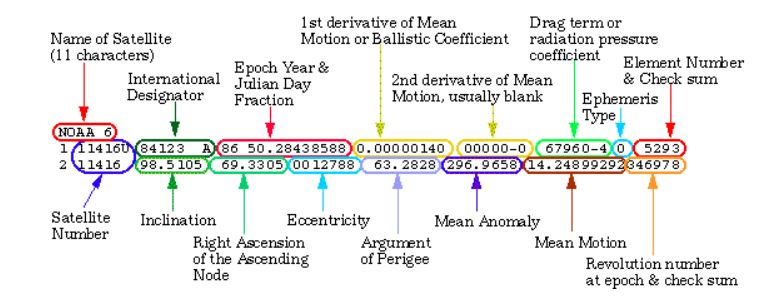
\includegraphics[width=0.7\linewidth]{tle_nasa}
		\caption{TLE with descriptions\cite{NASATLE}.}
		\label{fig:tlenasa}
	\end{figure}
	
	\begin{enumerate}\singlespacing
		\item \textbf{Name of Satellite:} NOAA 6
		
		This is the name of the satellite. In this example it is NOAA 6.
		\item 	\textbf{International Designator:} 84123 A
		
		This number shows the last two digets of the launch year and what number launch of that year it was. In this example it is 84 123 A. The satellite was launched in the year 1984 and it was the 124th launch of the year. The A means that it was the first object that came from the launch. %\textcolor{red}{Check this is right}
		
		\item \textbf{Epoch Date and Julian Date Fraction:} 86 50.28438588
		
		The Epoch date shows the year this TLE was made and the Julian Date fraction is the number of days in said year. 
		
		\item \textbf{First Derivative of Mean Motion:} 0.00000140
		
		This is the daily rate of change of number of revolutions the object completes per day divided by two. This is also called the ballistic coefficient.\cite{NASATLE} It's units are $\frac{rev}{day^2}$. 
		
		\item \textbf{Second Derivative of Mean Motion:} 00000-0
		
		This is the second derivative of mean motion divided by six, with units of $\frac{rev}{day^3}$.
		
		\item \textbf{Drag term or B* Term: }6970-4
		
		Of the terms given here, the B* term is the least heard of. It is a way of modeling drag on orbiting objects in propagation models.  
		Aerodynamic drag is given by the following equation:
		\begin{equation}
		F_D = \frac{1}{2}\rho C_d A v^2
		\end{equation}
		Where $A$ is the area, $C_d$ is the drag coefficient, $v$ the velocity, and $\rho$ is the fluid density. From Newton's second law
		%\begin{equation}
		%F = m\times a
		%\end{equation}
		the acceleration due to the force of drag is 
		\begin{equation}
		F = m\times a\rightarrow a_D=\frac{F_D}{m}=\frac{\rho C_d A v^2}{2m}=\frac{ C_d A}{m}\times\frac{\rho v^2}{2}
		\end{equation}
		The ballistic coefficient and starred ballistic coefficient are given by:
		%\begin{equation}
		%B=\frac{ C_d A}{m}
		%\end{equation}
		%The starred ballistic coefficient is then
		\begin{equation}
		B=\frac{ C_d A}{m}\rightarrow B^{*} = \frac{\rho_0 B}{2}=\frac{\rho_0 C_d A}{2m}
		\end{equation}
		This turns the equation for acceleration due to drag into \cite{celestrak_TLE_FAQ}\cite{castor2_BSTAR}
		\begin{equation}
		a_D=\frac{\rho}{\rho_0}B^{*} v^2
		\end{equation}
		%\textcolor{red}{Possibly not needed maybe take out. }\par 
		\item \textbf{Element Set Number :} 529
		The element set number represents how many TLEs have been generated for this object as of the current TLE.
		
		\item \textbf{Check Sum: } 3
		
		The checksum is a bit of data used to detect errors that occur during  transmission.
		
		\item \textbf{Satellite Number: } 11416U
		
		This is the Satellite Catalog Number and designation of the object. A U means unclassified. 
		
		\item \textbf{Inclination (degrees): }98.5105
		
		%This is one of the orbital elements.
		\item \textbf{Right Ascension of the Ascending Node (degrees): }69.3305
		
		%This is one of the orbital elements.
		
		\item \textbf{Eccentricity: } 0012788
		
		%This is one of the orbital elements.
		
		\item \textbf{Argument of Perigee (degrees): }63.2828
		
		%This is one of the orbital elements.
		
		\item \textbf{Mean Anomaly (degrees): }296.9658
		
		These four terms are all orbital elements.
		%Inclination, RAAN, Eccentricity, Argument of Perigee, and Mean Anomaly are all orbital elements.
		
		\item \textbf{Mean Motion: } 14.24899292
		
		This is the orbits per day the object completes. There are always 8 digits after the decimal place. 
		
		\item \textbf{Revolution Number: } 34697
	
		This is the number of revolutions the object has completed as of the TLE's generation.
		
		\item \textbf{Checksum: }8
		
		This is the checksum for the second line.
		
		
		
	\end{enumerate}\doublespacing

\par 
	A second example TLE is given in Appendix 2. The format in Appendix 2 is more compact and useful as a quick reference for TLEs. 
	\iffalse
\newpage	
	\singlespacing
A second example is given below, this time with references to the position of values, for extraction. The line under the dashes is the reference number line. The example TLE is described in table  \ref{tab:TLE_Desc}. This page is a useful compact summary of a TLE.
	\begin{verbatim}
	ISS (ZARYA)
	1 25544U 98067A   04236.56031392  .00020137  00000-0  16538-3 0  9993
	2 25544  51.6335 344.7760 0007976 126.2523 325.9359 15.70406856328906
	----------------------------------------------------------------------
	1234567890123456789012345678901234567890123456789012345678901234567890   
	1         2         3         4         5         6         7
	
	\end{verbatim}%
%	Table describes the second example TLE. 
	% Please add the following required packages to your document preamble:
	% \usepackage{graphicx}
	% \usepackage[table,xcdraw]{xcolor}
	% If you use beamer only pass "xcolor=table" option, i.e. \documentclass[xcolor=table]{beamer}
	
	% Please add the following required packages to your document preamble:
	% \usepackage{graphicx}
	% \usepackage[table,xcdraw]{xcolor}
	% If you use beamer only pass "xcolor=table" option, i.e. \documentclass[xcolor=table]{beamer}
		\begin{table}[h!]
		\centering
		\caption{Description of  example TLE\cite{SpaceTrackTLE}}
		\label{tab:TLE_Desc}
		\resizebox{\textwidth}{!}{%
			\begin{tabular}{|l|l|l|}
				\hline
				\multicolumn{3}{|l|}{\textbf{Line 0}}                                                                                                                               \\ \hline
				\rowcolor[HTML]{333333} 
				{\color[HTML]{FFFFFF} \textbf{Columns}} & {\color[HTML]{FFFFFF} \textbf{Example}} & {\color[HTML]{FFFFFF} \textbf{Description}}                                     \\ \hline
				1-24                                    & ISS (ZARYA)                             & The common name for the object based on information from the Satellite Catalog. \\ \hline
				\multicolumn{3}{|l|}{\textbf{Line 1}}                                                                                                                               \\ \hline
				\rowcolor[HTML]{333333} 
				{\color[HTML]{FFFFFF} \textbf{Columns}} & {\color[HTML]{FFFFFF} \textbf{Example}} & {\color[HTML]{FFFFFF} \textbf{Description}}                                     \\ \hline
				1                                       & 1                                       & Line Number                                                                     \\ \hline
				3-7                                     & 25544                                   & Satellite Catalog Number                                                        \\ \hline
				8                                       & U                                       & Elset Classification                                                            \\ \hline
				10-11                                   & 98                                      & International Designator (Last two digits of launch year)                       \\ \hline
				12-14                                   & 067                                     & International Designator (Launch number of the year)                            \\ \hline
				15-17                                   & A                                       & International Designator (Piece of the launch)                                  \\ \hline
				19-32                                   & 04                                      & Epoch Year (last two digits of year)                                            \\ \hline
				21-32                                   & 236.56031392                            & Epoch (day of the year and fractional portion of the day)                       \\ \hline
				34-43                                   & .00020137                               & 1st Derivative of the Mean Motion with respect to Time                          \\ \hline
				45-52                                   & 00000-0                                 & 2nd Derivative of the Mean Motion with respect to Time (decimal point assumed)  \\ \hline
				54-61                                   & 16538-3                                 & B* Drag Term                                                                    \\ \hline
				63                                      & 0                                       & Element Set Type                                                                \\ \hline
				65-68                                   & 999                                     & Element Number                                                                  \\ \hline
				69                                      & 3                                       & Checksum                                                                        \\ \hline
				\multicolumn{3}{|l|}{\textbf{Line 2}}                                                                                                                               \\ \hline
				\rowcolor[HTML]{333333} 
				{\color[HTML]{FFFFFF} \textbf{Columns}} & {\color[HTML]{FFFFFF} \textbf{Example}} & {\color[HTML]{FFFFFF} \textbf{Description}}                                     \\ \hline
				1                                       & 2                                       & Line Number                                                                     \\ \hline
				3-7                                     & 25544                                   & Satellite Catalog Number                                                        \\ \hline
				9-16                                    & 51.6335                                 & Orbit Inclination (degrees)                                                     \\ \hline
				18-25                                   & 344.7760                                & Right Ascension of Ascending Node (degrees)                                     \\ \hline
				27-33                                   & 0007976                                 & Eccentricity (decimal point assumed)                                            \\ \hline
				35-42                                   & 126.2523                                & Argument of Perigee (degrees)                                                   \\ \hline
				44-51                                   & 325.9359                                & Mean Anomaly (degrees)                                                          \\ \hline
				53-63                                   & 15.70406856                             & Mean Motion (revolutions/day)                                                   \\ \hline
				64-68                                   & 32890                                   & Revolution Number at Epoch                                                      \\ \hline
				69                                      & 6                                       & Checksum                                                                        \\ \hline
			\end{tabular}%
		}
	\end{table}
	
	

		\doublespacing
		\fi
  
	

	\section{NORAD Space-Track}	
	Now we understand the format of data that is available (the Two-Line Element set) and the format we want the data to be in (the orbital elements), the next thing to do is get the data. We want a source of TLEs for objects in space. Fortunately, there is one.\par 
	As well as tracking one S. Claus every December 24th\cite{noradSC},  NORAD also tracks all objects currently in space. This is done through the Space Surveillance Network\cite{ssncltrak}. The process of TLE gathering and updating is somewhat shadowy. \cite{vallado2012two} What is known is that observations are collected multiple times per day at the Joint Space Operations Center (JSPOC) which is operated by the US Air Force Space Command (AFSPC). Then the unclassified TLEs are passed on for public release via the website space-track.org. Objects in space are tracked by radar systems (conventional and phased array) as well as the Ground-Based Electro-Optical Deep Space Surveillance system (GEODSS)\cite{GEODSS}.
	

	
	%Describe the site
	%desribe the SATCAT, then the TLE query
	
	\subsection{Space-Track.org}
	In their own words, Space-Track.org  ``promotes space flight safety, protection of the space environment and the peaceful use of space worldwide by sharing space situational awareness services and information with U.S. and international satellite owners/operators, academia and other entities."\cite{SpaceTrackHome}\par 
	Information about objects in space may be found the website space-track.org. Space-track is the main source for orbital data, though some are also available from the website celestrak.com. Of the two space-track has far more information and better methods of access.  "Space-Track.org is managed, maintained and administered by JFSCC"\cite{SpaceTrackLegend}.   %\textcolor{red}{Put more information about the website here}.\par 
	Space-track allows information to be downloaded manually from the TLE search \cite{SpaceTrackTLE} or the satellite catalog search \cite{SpaceTrackSATCAT}. While these are useful tools the code needs a way to automatically download data. Fortunately space-track also has an API that allows queries. 
	\subsection{Space-Track Query}
	An application programming interface or API is a set of methods that allow simple communication between different codes. The Space-Track API allows for programs to send requests for data on objects in space. It is limited to less than 20 requests per minute and less than 200 requests per hour. 
	
	
	The API works by building an API similar to the following URL:
	
	\url{https://www.space-track.org/basicspacedata/query/class/boxscore/} 
	
	Where: 

	\begin{itemize}	\singlespacing
		\item Base URL: https://www.space-track.org/
		
		\item Request Controller: basicspacedata
		\item Request Action: query
		\item Predicate Value Pairs: class/boxscore/
	\end{itemize}
\doublespacing
The only publicly available Request Controller is basicspacedata. The expandedspacedata controller requires SSA Sharing Agreements \cite{SpaceTrackAPI}. The first two sections of the URL will never change. What will changes is the query, the class, and the boxscore. The request classes that are of interest to this thesis are in table \ref{tab:reqClass}.\par

\singlespacing
\begin{table}[H]
	\caption{Request Classes of Interest\cite{SpaceTrackAPI}}
	\label{tab:reqClass}
	\begin{tabular}{|l|p{13.5cm}|}
		\hline
		Class Name     & Class Description                                                                                                                                                                                                                                                                                                                                                                                                                                                                                                                                                                                                                                \\ \hline
		tle            & Historical record of orbital element sets (Two-Line Elements). Additional metadata columns are available so that users can filter their queries by these values, downloading only the data they need. Shown in html, csv, and xml formats, these additional columns include: object\_name, object\_type, semi-major axis, period, apogee, perigee, and file. NOTE: There are over 97 million TLEs in the database. The user is strongly advised to limit their API queries by OBJECT\_NUMBER / NORAD\_CAT\_ID AND an epoch range such as "$>$now-30" to avoid "Query range out of bounds" errors.\\ \hline

		satcat         & Satellite Catalog Information. The "CURRENT" predicate indicates the most current catalog record with a 'Y'. All older records for that object will have an 'N'.\\ \hline      
		
		omm            & Orbit Mean-Elements Message (OMM)Keplerian element format that complies with CCSDS Recommended Standard 502.0-B-2 \\ \hline                                                                                                                                                                                                                                                                                                                                                                                                                                                                           
	\end{tabular}
\end{table}\doublespacing

The Orbit Mean-Elements Message was not used in this thesis because it could not handle large groups of requests. However because it directly returns the Keplerian elements, it may be useful if the API functionality is improved in the future. As a result the TLE and satcat classes are the only classes used in this code. The predicate values pairs may be specified by using REST Operators. The REST Operators that can be used are seen in table \ref{tab:restOP}

\begin{table}[H]\singlespacing
	\caption{REST Operators\cite{SpaceTrackAPI}}
	\label{tab:restOP}
	\begin{tabular}{|l|p{13.5cm}|}
		\hline
		Operator                  & Description                                                                                                                                                                                                                                                                         \\ \hline
		\textgreater{}            & Greater Than (alternate is \%3E)                                                                                                                                                                                                                                                    \\ \hline
		\textless{}               & Less Than (alternate is \%3C)                                                                                                                                                                                                                                                       \\ \hline
		\textless{}\textgreater{} & Not Equal (alternate is \%3C\%3E)                                                                                                                                                                                                                                                   \\ \hline
		,                         & Comma Delimited 'OR' (ex. 1,2,3)                                                                                                                                                                                                                                                    \\ \hline
		--                        & Inclusive Range (ex. 1--100 returns 1 and 100 and everything in between)Date ranges are expressed as YYYY-MM-DD\%20HH:MM:SS--YYYY-MM-DD\%20HH:MM:SS or YYYY-MM-DD--YYYY-MM-DD                                                                                                       \\ \hline
		null-val                  & Value for 'NULL', can only be used with Not Equal (\textless{}\textgreater{}) or by itself.                                                                                                                                                                                         \\ \hline
		$\sim$$\sim$              & "Like" or Wildcard search. You may put the $\sim$$\sim$before or after the text; wildcard is evaluated regardless of location of $\sim$$\sim$in the URL.For example, $\sim$$\sim$OB will return 'OBJECT 1', 'GLOBALSTAR', 'PROBA 1', etc.                                           \\ \hline
		\textasciicircum{}        & Wildcard after value with a minimum of two characters. (alternate is \%5E) The wildcard is evaluated after the text regardless of location of \textasciicircum in the URL. For example, \textasciicircum{}OB will return 'OBJECT 1', 'OBJECT 2', etc. but not 'GLOBALSTAR'           \\ \hline
		now                       & Variable that contains the current system date and time. Add or subtract days (or fractions thereof) after 'now' to modify the date/time, e.g. now-7, now+14, now-6.5, now+2.3. Use \textless{},\textgreater{},and -- to get a range of dates; e.g. \textgreater{}now-7, now-14--now \\ \hline
	\end{tabular}
\end{table}\doublespacing

The REST Predicates are seen in table \ref{tab:restP}


\begin{table}[H]\singlespacing
	\caption{REST Predicates\cite{SpaceTrackAPI}}
	\label{tab:restP}
	\begin{tabular}{|p{4cm}|p{11.5cm}|}
		\hline
		REST Predicates                & REST Description                                                                                                                                                                                                                                                           \\ \hline
		class/classname                & Class of data message requested from the API. Required for all operations.                                                                                                                                                                                                 \\ \hline
		predicates/p1, p2,...          & Comma-separated list of predicates to be returned as the result. Can also be set to 'all' or omitted entirely for default behavior of returning all predicates.                                                                                                            \\ \hline
		metadata/true                  & Includes data about the request (total \# of records, request time, etc); ignored when used with tle, 3le, and csv formats.                                                                                                                                                \\ \hline
		limit/x(,x?)                   & Specifies the number of records to return. Takes an integer for an argument, with an optional second argument to specify offset. For example, /limit/10/ will return the first 10 records; /limit/10,5/ will show 10 records starting after record \#5 (rows 6 through 15) \\ \hline
		orderby/predicate (asc?|desc?) & Allows ordering by a predicate (column), either ascending or descending, with asc/desc separated from the predicate by a space. Multiple Orderings are supported, separating the pairs of predicate and asc/desc by commas (e.g. http://.../DECAY desc,APOGEE desc/...)    \\ \hline
		distinct/true                  & Removes duplicate rows.                                                                                                                                                                                                                                                    \\ \hline
		format/xxxx                    & Specifies return format, can be: json, xml, html, csv, tle, 3le, kvn, or stream. See below for additional information. If no format is specified, the default is JSON                                                                                                      \\ \hline
		emptyresult/show               & Queries that return no data will show 'NO RESULTS RETURNED' instead of the default blank page                                                                                                                                                                              \\ \hline
	\end{tabular}
\end{table}\doublespacing


Finally the data returned may be in the formats seen in table \ref{tab:dataFormat}

\begin{table}[H]\singlespacing
	\caption{Available Data Formats\cite{SpaceTrackAPI}}
	\label{tab:dataFormat}
	\begin{tabular}{|l|p{9cm}|}
		\hline
		Format                             & Request Rules                                                                                                                                                                                                                                                                                                                                                                                                                                                                             \\ \hline
		eXtensible Markup Language (xml)  & No special request rules. For CDM request class, shows CCSDS-compliant format.                                                                                                                                                                                                                                                                                                                                                                                                            \\ \hline
		JavaScript Object Notation (json) & Preferred format, no special request rules.                                                                                                                                                                                                                                                                                                                                                                                                                                               \\ \hline
		HyperText Markup Language (html)  & Not recommended for machine parsing. No special request rules.                                                                                                                                                                                                                                                                                                                                                                                                                            \\ \hline
		Comma-Separated Values (csv)      & Due to the limitations of the CSV specification, requesting CSV formatted data does not allow for transmission of metadata; metadata concerning the request will need to be gathered through one of the other formats prior to requesting CSV.                                                                                                                                                                                                                                            \\ \hline
		Two-Line Element Set (tle)        & To get traditionally-formatted TLE data, request the 'tle', 'tle\_latest', or 'tle\_publish' class. We recommend that you omit predicates from URLs that use tle format. If you do include predicates, it must include line 1 \& 2 like this: ``/predicates/TLE\_LINE1,TLE\_LINE2/". Like CSV, tle format ignores /metadata/true/ REST Predicate.                                                                                                                                          \\ \hline
		Three-Line Element Set (3le)      & The format adds TLE\_LINE0 or the ``Title line", a twenty-four character name, before the traditional Two Line Element format. The 3le format defaults to include a leading zero so that you can easily find the object name via scripts. If you do not want the leading zero, you should include this in your URL to show the OBJECT\_NAME instead of TLE\_LINE0: ``/predicates/OBJECT\_NAME,TLE\_LINE1,TLE\_LINE2/". Like CSV and tle, 3le format ignores /metadata/true/ REST Predicate. \\ \hline
		Key=Value Notation (kvn)          & Key=Value Notation format, currently for use exclusively with CDM Class. Incompatible with /metadata/true/.                                                                                                                                                                                                                                                                                                                                                                               \\ \hline
		File Stream (stream)              & File Stream format, currently for use exclusively with download class.                                                                                                                                                                                                                                                                                                                                                                                                                    \\ \hline
	\end{tabular}
\end{table}\doublespacing
	%\subsection{SatCat?}
	
	
	\subsection{Code Queries}
	Using the following rules, the code generates URLs that query space-track for the relevant information. The first URL is used to acquire the relevant satcat IDs for space debris. It is as follows:\par 
	
	\url{https://www.space-track.org/basicspacedata/query/class/satcat/OBJECT_TYPE/debris/RCS_SIZE/small/LAUNCH_YEAR/>1990/orderby/DECAY asc/format/csv/metadata/false}
	
	
	%\url{https://www.wikibooks.org}
	%\href{https://www.wikibooks.org}{Wikibooks home}
	
	%\href{https://www.space-track.org/basicspacedata/query/class/satcat/OBJECT_TYPE/debris/RCS_SIZE/small/LAUNCH_YEAR/>1990/orderby/DECAY asc/format/csv/metadata/false}{https://www.space-track.org/basicspacedata/query/class/satcat/OBJECT\_TYPE/debris/RCS\_SIZE/small/LAUNCH\_YEAR/$>$1990/orderby/DECAY asc/format/csv/metadata/false}
	
	Where 1990 is the launch year, and should be replaced by the year the debris was launched in. This is the best way of controlling how much debris the user gets. Setting a launch year of 1960 will obviously included all small debris (debris that is less than 10 cm$^2$ cross section), while setting a launch year of 2018 would return very little debris. It is advisable to run test cases with small debris before performing operations on all available debris. A detailed walkthrough of the URL may be seen in table \ref{tab:url1}.\par 
	%This url will return the satcat Ids as seen by the ``class/satcat''. It will return them in a csv format as seen by the ``format/csv'' and it will only select small debris, as seen by the ``RCS\_SIZE/small''.\par 
	
	%Unpacking this:
	
	\begin{table}[H]\singlespacing
		\caption{Detailed Description of First URL}
		\label{tab:url1}
		\begin{tabular}{|p{6cm}|p{10cm}|}
			\hline
			Section of URL & Description \\ \hline
			https://www.space-track.org/basicspacedata/query/ & This is the base URL. \\ \hline
			class/satcat/ & The class of the data will be the satcat Ids. \\ \hline
			OBJECT\_TYPE/debris/ & The type of object this URL is looking for is debris \\ \hline
			/CS\_SIZE/small/ & The URL is looking for debris classified as small \\ \hline
			LAUNCH\_YEAR/$>$\textbf{launchYear}/ & The debris is limited by the provided launch year. \\ \hline
			orderby/DECAY asc/ & The debris are ordered by their decay. This order is not relevant, and only included because it is a necessary part of the query. The IDs are sorted small to large after the post request. \\ \hline
			format/csv/metadata/false & Finally the format of the data returned is set to be a csv. The metadata of the request is not given. \\ \hline
		\end{tabular}
	\end{table}\doublespacing
	
	
	The second URL is later used to return the TLEs from given satcat Ids. It follows the following format:\par 
	
	
		\url{	https://www.space-track.org/basicspacedata/query/class/tle_latest/NORAD_CAT_ID/ 43543,43544,43555/orderby/ORDINAL%20asc/limit/3/format/tle/metadata/false
		}
	%https://www.space-track.org/basicspacedata/query/class/tle\_latest/NORAD\_CAT\_ID/\newline 43543,43544,43555/orderby/ORDINAL\%20asc/limit/\textbf{numTLE}/format/tle/metadata/false
	
	A detailed description of this URL may be seen in table \ref{tab:tle2url}
	
	\begin{table}[H]\singlespacing
		\caption{Detailed Description of Second URL}
		\label{tab:tle2url}
		\begin{tabular}{|p{6cm}|p{10cm}|}
			\hline
			Section of URL                                    & Description                                                                                                                                                                                                                                     \\ \hline
			
			https://www.space-track.org/basicspacedata/query/ & This is the base URL, unchanged from the previous example.                                                                                                                                                                                      \\ \hline
			class/tle\_latest/                                & The class of the data will be the latest TLEs.                                                                                                                                                                                                  \\ \hline
			NORAD\_CAT\_ID/                                   & The data will come from the following NORAD CAT IDs.                                                                                                                                                                                            \\ \hline
			43543,43544,43555/                                & The NORAD CAT IDs that have been requested. Normally the code will request many of them, to make this easy to read only three IDs have been requested in this example.                                                                          \\ \hline
			orderby/ORDINAL\%20asc/                           & The TLEs will be in ascending order. Ascending or descending order does not matter as the order is changed by MATLAB soon after.                                                                                                                \\ \hline
			limit/\textbf{numberOfTLEs}/            & This is the number of TLEs to be returned. The number of TLEs should be the same as the number of NORAD CAT IDs provided. This ensures that only one TLE per CAT ID is returned and only the most recent TLE for a piece of debris is returned. In this case it will be 3.\\ \hline
			format/tle/metadata/false                         & Finally the format of the data returned is set to be TLEs. The metadata of the request is not given.                                                                                                                                            \\ \hline
		\end{tabular}
	\end{table}\doublespacing

\subsection{Post Requests}
Once the query URL has been created the next step is using the URL to obtain data. A human may simply type the query URL into a browser. For example typing the following URL into an Internet browser: 

\url{https://www.space-track.org/basicspacedata/query/class/tle/format/tle/NORAD_CAT_ID/25544/orderby/EPOCH%20desc/limit/1}
	
	Provides the result seen in figure \ref{fig:isstle}. This is of course the most recent TLE for the ISS.
	
	\begin{figure}[H]
		\centering
		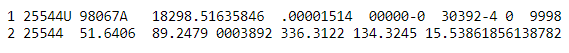
\includegraphics[width=0.7\linewidth]{ISS_tle}
		\caption{TLE for ISS from query URL}
		\label{fig:isstle}
	\end{figure}

However space-track requires a username and password. A browser that humans use saves this information. Typing this URL in without the username and password saved will redirect to the front page of space-track. For MATLAB to use these query URLs and provied a username and password a POST request is needed. \par 

A POST method is a way of requesting data by providing information that would be entered into HTML fields, such as a a username or password \cite{postRef}. In effect the POST request is able to to go to a website, fill out and fields needed (such as username and password fields) and retrive the desired data. In MATLAB a post request looks like this:	
	
\singlespacing
\begin{lstlisting}
function postOutput = examplePostRequest(username,password,timeOutVal)
	baseURL='https://www.space-track.org/'; % base URL
	logURL=[baseURL,'ajaxauth/login']; % login URL
	querySatcatURL=[baseURL,'basicspacedata/query/class/tle/format/', 'tle/NORAD_CAT_ID/25544/orderby/EPOCH%20desc/limit/1']; % query URL
	post={'identity',username, 'password', password, 'query', querySatcatURL}; % create post request
	postOutput=urlread(logURL,'Post',post,'Timeout',timeOutVal); % runs and gets the output of the post request
end 
\end{lstlisting}
\doublespacing
The output of this post request is 

\begin{figure}[H]
	\centering
	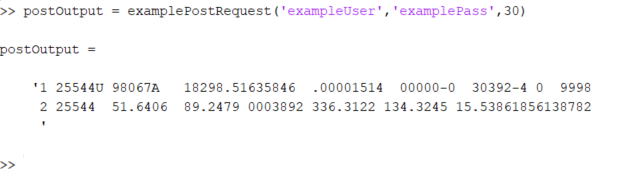
\includegraphics[width=0.7\linewidth]{ISS_tle_Post}
	\caption{Output of examplePostRequest.m}
	\label{fig:isstlepost}
\end{figure}

This POST request uses the MATLAB function urlread to send the username, password, query URL, and a timeout value. The time out value is the length of time in seconds the code will wait for a response from the server. It returns a char with a TLE for the ISS. This type of POST request is implemented in this thesis's code. 

	%\begin{itemize}\singlespacing
	%	\item 	https://www.space-track.org/basicspacedata/query/ : This is the base URL, unchanged from the previous example.
	%	\item class/tle\_latest/ : The class of the data will be the latest TLEs
	%	\item NORAD\_CAT\_ID/ : The data will come from the following NORAD CAT IDs
		%\item 43543,43544,43555/ : The NORAD CAT IDs that have been requested. Normally the code will request many of them, to make this easy to read only three IDs have been requested in this example.
	%	\item orderby/ORDINAL\%20asc/ : The TLEs will be in ascending order. Ascending or descending order does not matter as the order is changed by MATLAB soon after.
	%	\item  limit/\textbf{numTLE} : This is the number of TLEs to be returned. The number of TLEs should be the same as the number of NORAD CAT IDs provided. This ensures that only one TLE per CAT ID is returned and only the most recent TLE for a peace of debris is returned.
	%	\item format/tle/metadata/false : Finally the format of the data returned is set to be TLEs. The metadata of the request is not given. 
	%\end{itemize}\doublespacing
	%\begin{align}
	%\underbrace{\text{space-track.org/basicspacedata/query/}}_\text{Base URL, unchanged}	\underbrace{\text{class/tle\_latest/NORAD\_CAT\_ID/}}_\text{The class of the data will be the latest TLE from the given NORAD CAT Ids}\nonumber
	%\end{align}
	\section{Code Overview}
	The code obtains orbital data for space debris depending on what variables the user has inputted, such as the launch year of the debris or how recent the data should be.
	First the code ascertains what data is already available. It checks to see if there is a .mat file for the SATCAT. This is simply a file that contains the catalog ids of the debris. If this file does not exist then the code has not been run for the current parameters, and the code will be run. \par 
	The code will also check to see if there is a TLE .mat file. If this file exists the code then checks when the file was created. Depending on user variables, the code may consider the information to be out of date, will rerun everything. However if the TLE .mat file is recent, then the code will load the current debris data into the workspace.\par 
	Assuming that the code detects that it has no data, or the data is out of date the code will work in the following steps\par 
	\begin{enumerate}
		\item The desired NORAD satellite catalog ids will be collected with the get\_SATCAT.m file. These ids are determined by user variables such as launch date. The code downloads them as a csv, strips things like quotation marks away, and sorts the ids in order.
		\begin{itemize}
			\item if a SATCAT .mat file exists and is recent this step is skipped.
		\end{itemize}  
	\item The code then begins to loop through the array of Ids. It enters an error catch to handle url time outs. 
		\begin{itemize}
		\item Within this loop the code then downloads the TLEs from the satellite ids. The TLEs are stored in a string. It does this in groups that have their size determined by the user. A large group size may risk url timeouts, but a small group size will result in a long run time.
		\item The TLEs are then parsed, the TLEs are turned into usable orbital information, and saved as an array in MATLAB.
		\item When the loop has run through all the Ids, the array of data is saved as a .mat file wit the date of it's creation.
	\end{itemize} 
\item Now the array of debris data is ready. A copy is saved with a header listing what each collum represents. Another is sent to an orbit visualization file. 

\item  It should be noted that not all TLEs requested will be provided. So if the code requests TLEs of objects with a id from 1000 to 1100 and expects 100 TLEs, but some are classified, then duplicated TLEs less than 100 TLEs will be returned. The user now has a usable list of space debris and their orbital elements.
	
		%\item The code then downloads the TLEs as .txt files from the satellite ids. It does this in groups that have their size determined by the user. 
		%\item The .txt files are then parsed, the TLEs are turned into usable orbital information, and saved as an array in MATLAB. This is done in the readTLE\_txt.m file.
		%\item Finally the array of debris information is sorted in order of satellite id and duplicate rows are removed. It should be noted that not all TLEs requested will be provided. So if the code requests TLEs of objects with a id from 1000 to 1100 and expects 100 TLEs, but some are classified, then duplicated TLEs will be returned to make 100 TLEs. As such these duplicates must be removed. The final array is stored in a .mat file with it's date of creation noted. The user now has a usable list of space debris and their orbital elements.
	\end{enumerate}

	What now follows is a more in depth explanation of each file. 
		\subsection{VarStore.m}
		This is a file where a few important variables are stored. It allows the user to only have to edit one file to change the code's operation.
		\subsection{UserPass.m}
		This file is where the username and password for space-track.org are stored. This is kept separate from the other code to ensure privacy of username and password. 
		\subsection{MASTER\_TLE.m}
		This file is the master file for the Two Line Element MATLAB files. Running it will run all of the associated MATLAB files. These MATLAB files take some time to run, so it may be convenient to alter the range of data operated on by MASTER\_TLE.m in VarStore.m
		\subsection{get\_SATCAT.m}
		Get\_SATCAT.m is the MATLAB file that gets the satellite catalog  numbers of all orbital debris launched after a given year and with the “RCS\_SIZE” value equal to “SMALL”. The first URL described previously is used here. The Launch Year can be set by the values given by the user in VarStore.m The default launch year is set to 1990. Note that an earlier launch year will provide more data, and thus it will take more time to process. This may cause a time out error. Should this happen the timeOutVal in VarStore.m should be adjusted to be longer.\par 
		Once the SATCAT csv file has been acquired the file then formats it. The quotation marks that are around every entry are removed. The debris that have already deorbited are also removed. Finally the debris is sorted by NORAD Catoluge Id, and saved as a .mat file.
		The post request in the get\_SATCAT.m file was originally developed by Joao Encarnacao\cite{codeGETtle}
		%\subsection{get\_Multiple\_TLE\_from\_Id.m}
		%This file takes the Ids given in the .mat file and then obtains the Two Line Element files associated with the debris. It does this by saving the TLEs in .txt files. The number of TLEs grabbed at a time and saved in a .txt file is set by the user. It is not advised to go above 400, as that causes time out errors. \par 
		%Withing MASTER\_TLE.m, this code is surrounded by a a loop and a try/catch error. The loop runs through all the different blocks of TLEs. In the case of a time out the the try/catch will attempt to download the TLEs a second time.\par 
		%At this point in the code the space debris has had it's Two Line Element files saved to .txt files. This is the longest part of the code to run, but also with the .txt files saved, these functions need only be run once every few days. 

		%\subsection{readTLE\_txt.m}
		%This MATLAB file reads the .txt files and then converts the TLE format to the standard orbital elements stored in a .mat file. 
		%\subsection{check\_TLE\_Edit\_TLE.m}
		
		\subsection{get\_TLE\_from\_ID\_Manager.m}
		The purpose of get\_TLE\_from\_ID\_Manager.m is to act as a handler for function \newline get\_TLE\_from\_NorID.m. The code first checks to see if there exists a folder to store the data in, if there is not a folder is created. Then the code begins to run through the list of NORAD Ids. It sends these Ids to get\_TLE\_from\_NorID.m, receives the orbital element data from those Ids. 
		
		The code also contains an error handler. The most common problem with downloading large numbers of TLEs is a URL timeout may occur. Timeouts are easy for a human to deal with, they may be fixed by simply refreshing the web page. However for MATLAB, it is more difficult. The code deals with a URL timeout as follows:
		
		First the code detects the specific error thrown for URL timeouts. This error is caught, so the code does not stop running. Then the code gets the current location in the Id array the time out occurred at, and restarts at that spot. The effect of this is the same as refreshing a webpage that is not loading. 
		
		Once all the data has been collected for the given Ids, it is saved as a .mat file with the time that it was created.
		\subsection{get\_TLE\_from\_NorID.m}
		The purpose of get\_TLE\_from\_NorID.m is to download the TLEs from NORAD given Ids, and to save the TLEs as useful orbital elements. This function may be divided into two parts: the web interface for TLEs and the TLE to orbital element section. 
		
		The first part of the code creates a URL from the current set of Ids. This url is then used to download the TLEs. The TLEs are saved as a string within MATLAB.  
		
		In the next part of the code a loop goes through the TLE string. The information from these TLEs is saved as a matrix. Earlier versions of this projects code first downloaded all TLEs as .txt files and then parsed through the .txt files to get the orbital elements. However that was unnecessarily slow as MATLAB had to open each .txt file and read it's contents as opposed to reading the contents of a string already in the workspace. By constantly saving the results as a .mat file through out the operation of the code, there is no threat of data loss. 
		
			
		
		From each TLE the inclination (i), RA of ascending node ($\Omega$), eccentricity (e), argument of perigee ($\omega$), mean anomaly, and mean motion (n) may be acquired directly. From these values the other orbital elements may be calculated. 
		
		Period of rev:
		\begin{align}
		T=\frac{24\times60\times60}{n}
		\end{align}
		
		Semi-major axis:
		\begin{align}
		a=\left(\left(\frac{T}{2\pi}\right)^2 \times \mu_\text{earth}\right)^{(1/3)}
		\end{align}
		Where $\mu_\text{earth}$ is the standard gravitational parameter of earth: $3.986\times10^{14}$. Semi-minor axis:
		\begin{align}
		b=a\times\sqrt{1-e^2}
		\end{align}
		Perigee and Apogee:
		\begin{align}
		r_\text{per}=\left(1-e\right)\times a\\
		r_\text{ap}=\left(1+e\right)\times a
		\end{align}
		The code to parse the elements from the TLE was based off of Brett Pantalone's parse TLE code\cite{codeParseTLE}, modified to handle multiple TLEs from within the MATLAB workspace. 
		
		
	
	\section{Conclusion}
	The goal of this thesis was to create a program that can download the latest orbital elements needed to calculate the real time locations of space debris, given user inputted parameters. The information would be usable to someone who has taken a basic spaceflight mechanics class. 
	
	\subsection{Results of Code}
	When the code is run the result is a matrix of orbital elements, as seen in figure \ref{fig:matlaboutput}. 
	
	
	\begin{figure}[H]
		\centering
		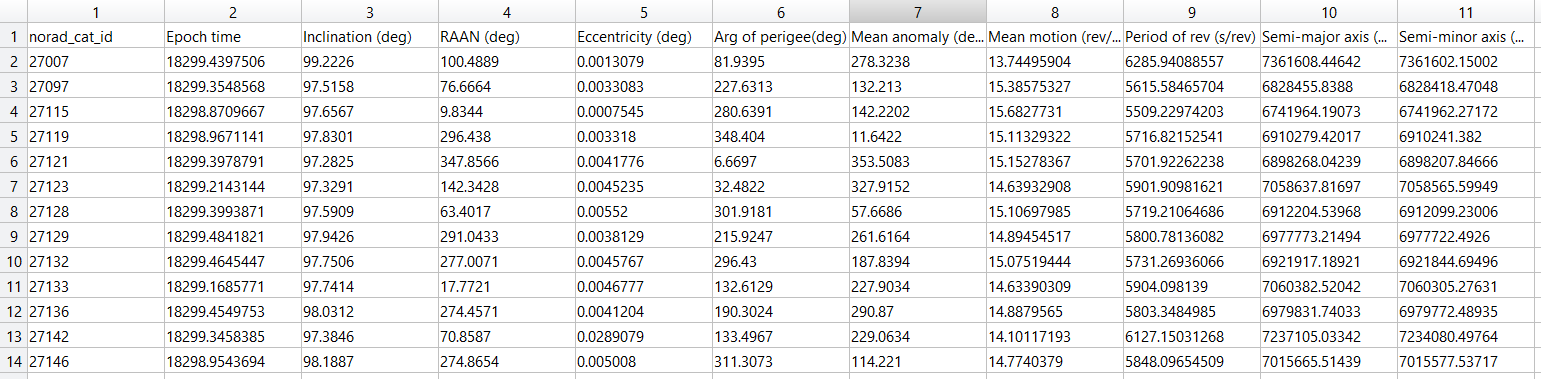
\includegraphics[width=0.7\linewidth]{MATLAB_output}
		\caption{MATLAB matrix resulting from code execution}
		\label{fig:matlaboutput}
	\end{figure}
	Compared to the data in figure \ref{fig:isstle} this is far easier for a person with basic orbital mechanics experience to use. A number of parameter sets have been provided for users to experiment with. 

%These results may be used to  may be used to catagorize data 
	
	%Once the data has been collected, the next step is to target possible orbits. Since OSCAR has a delta V of \textcolor{red}{Find delta V} inclination and plane changes are out of the question. What is desired is a number of debris in a plane with simialr inclanations.
	


\subsection{Future Work}

Now that data can be obtained the next step is to look at possible orbits to place OSCAR. Due to OSCAR's limited delta V inclination and plane changes are out of the question. Thus OSCAR should be inserted into a orbit which shares a inclination and RAAN with the most debris. The number of debris sorted by inclination and RAAN are seen in figure \ref{fig:ranninc}.

\begin{figure}[H]
	\centering
	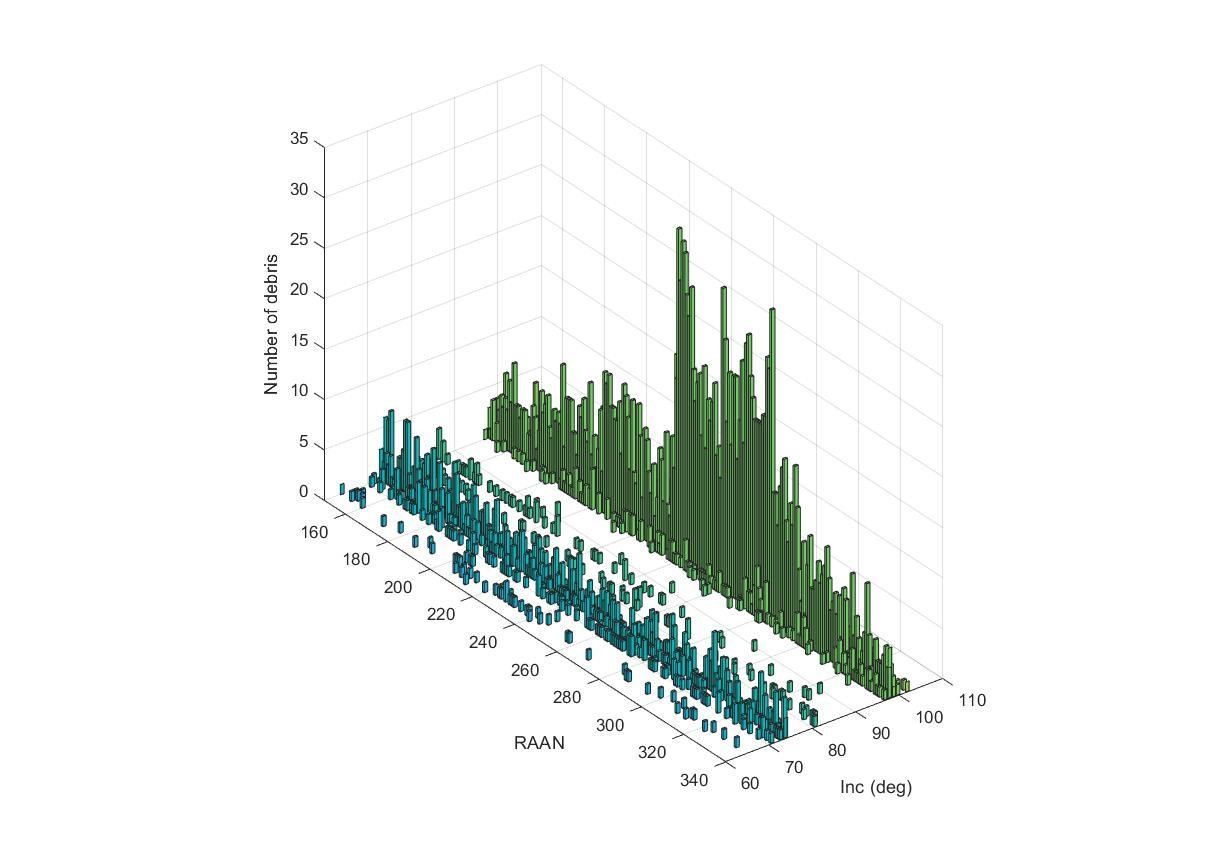
\includegraphics[width=0.7\linewidth]{rann_inc}
	\caption{Number of debris by inclination and RAAN}
	\label{fig:ranninc}
\end{figure}


The next step from this code would be to include propagation. The TLEs are for a given epoch, so to get the real time location prorogation from sgp4 is needed. Additionally the code should be developed to run autonomously on RPI computers, so there is a database of space debris that RPI controls.


	
		
		%--------------------------------------
		% References
		% -------------------------------------
		  \bibliographystyle{ieeetr} % specify bibliography style
		%\bibliographystyle{unsrt}
		\bibliography{ref}

		
		%-----------------------------------------------------------
		% Appendix
		%-----------------------------------------------------------
		\newpage
		\singlespacing
		\section{Appendix}
		\subsection{MATLAB Code}
		%\addcontentsline{toc}{section}{Appendix}
		
		\lstset{language=Matlab,%
			%basicstyle=\color{red},
			breaklines=true,%
			morekeywords={matlab2tikz},
			keywordstyle=\color{blue},%
			morekeywords=[2]{1}, keywordstyle=[2]{\color{black}},
			identifierstyle=\color{black},%
			stringstyle=\color{mylilas},
			commentstyle=\color{mygreen},%
			showstringspaces=false,%without this there will be a symbol in the places where there is a space
			numbers=left,%
			numberstyle={\tiny \color{black}},% size of the numbers
			numbersep=9pt, % this defines how far the numbers are from the text
			emph=[1]{for,end,break},emphstyle=[1]\color{red}, %some words to emphasise
			%emph=[2]{word1,word2}, emphstyle=[2]{style},    
		}
		
	\subsubsection{Master\_TLE.m}
	\lstinputlisting{C:/Users/Philip/Documents/GitHub/Thesis/latex_mat_files/Master_TLE.m}
	\subsubsection{get\_SATCAT.m}
		\lstinputlisting{C:/Users/Philip/Documents/GitHub/Thesis/get_SATCAT.m}
		\subsubsection{get\_TLE\_from\_ID\_Manager.m}
	\lstinputlisting{C:/Users/Philip/Documents/GitHub/Thesis/get_TLE_from_ID_Manager.m}
	
	\subsubsection{get\_TLE\_from\_NorID.m}
	\lstinputlisting{C:/Users/Philip/Documents/GitHub/Thesis/latex_mat_files/get_TLE_from_NorID.m}
		\newpage
	\subsection{TLE Reference Table}
	
	\singlespacing
	An example TLE is given below with references to the position of values. The line under the dashes is the reference number line. The example TLE is then described in table  \ref{tab:TLE_Desc}. This page is a useful compact summary of a TLE.
	\begin{verbatim}
	ISS (ZARYA)
	1 25544U 98067A   04236.56031392  .00020137  00000-0  16538-3 0  9993
	2 25544  51.6335 344.7760 0007976 126.2523 325.9359 15.70406856328906
	----------------------------------------------------------------------
	1234567890123456789012345678901234567890123456789012345678901234567890   
	1         2         3         4         5         6         7
	
	\end{verbatim}%
	%	Table describes the second example TLE. 
	% Please add the following required packages to your document preamble:
	% \usepackage{graphicx}
	% \usepackage[table,xcdraw]{xcolor}
	% If you use beamer only pass "xcolor=table" option, i.e. \documentclass[xcolor=table]{beamer}
	
	% Please add the following required packages to your document preamble:
	% \usepackage{graphicx}
	% \usepackage[table,xcdraw]{xcolor}
	% If you use beamer only pass "xcolor=table" option, i.e. \documentclass[xcolor=table]{beamer}
	\begin{table}[h!]
		\centering
		\caption{Description of  example TLE\cite{SpaceTrackTLE}}
		\label{tab:TLE_Desc}
		\resizebox{\textwidth}{!}{%
			\begin{tabular}{|l|l|l|}
				\hline
				\multicolumn{3}{|l|}{\textbf{Line 0}}                                                                                                                               \\ \hline
				\rowcolor[HTML]{333333} 
				{\color[HTML]{FFFFFF} \textbf{Columns}} & {\color[HTML]{FFFFFF} \textbf{Example}} & {\color[HTML]{FFFFFF} \textbf{Description}}                                     \\ \hline
				1-24                                    & ISS (ZARYA)                             & The common name for the object based on information from the Satellite Catalog. \\ \hline
				\multicolumn{3}{|l|}{\textbf{Line 1}}                                                                                                                               \\ \hline
				\rowcolor[HTML]{333333} 
				{\color[HTML]{FFFFFF} \textbf{Columns}} & {\color[HTML]{FFFFFF} \textbf{Example}} & {\color[HTML]{FFFFFF} \textbf{Description}}                                     \\ \hline
				1                                       & 1                                       & Line Number                                                                     \\ \hline
				3-7                                     & 25544                                   & Satellite Catalog Number                                                        \\ \hline
				8                                       & U                                       & Elset Classification                                                            \\ \hline
				10-11                                   & 98                                      & International Designator (Last two digits of launch year)                       \\ \hline
				12-14                                   & 067                                     & International Designator (Launch number of the year)                            \\ \hline
				15-17                                   & A                                       & International Designator (Piece of the launch)                                  \\ \hline
				19-32                                   & 04                                      & Epoch Year (last two digits of year)                                            \\ \hline
				21-32                                   & 236.56031392                            & Epoch (day of the year and fractional portion of the day)                       \\ \hline
				34-43                                   & .00020137                               & 1st Derivative of the Mean Motion with respect to Time                          \\ \hline
				45-52                                   & 00000-0                                 & 2nd Derivative of the Mean Motion with respect to Time (decimal point assumed)  \\ \hline
				54-61                                   & 16538-3                                 & B* Drag Term                                                                    \\ \hline
				63                                      & 0                                       & Element Set Type                                                                \\ \hline
				65-68                                   & 999                                     & Element Number                                                                  \\ \hline
				69                                      & 3                                       & Checksum                                                                        \\ \hline
				\multicolumn{3}{|l|}{\textbf{Line 2}}                                                                                                                               \\ \hline
				\rowcolor[HTML]{333333} 
				{\color[HTML]{FFFFFF} \textbf{Columns}} & {\color[HTML]{FFFFFF} \textbf{Example}} & {\color[HTML]{FFFFFF} \textbf{Description}}                                     \\ \hline
				1                                       & 2                                       & Line Number                                                                     \\ \hline
				3-7                                     & 25544                                   & Satellite Catalog Number                                                        \\ \hline
				9-16                                    & 51.6335                                 & Orbit Inclination (degrees)                                                     \\ \hline
				18-25                                   & 344.7760                                & Right Ascension of Ascending Node (degrees)                                     \\ \hline
				27-33                                   & 0007976                                 & Eccentricity (decimal point assumed)                                            \\ \hline
				35-42                                   & 126.2523                                & Argument of Perigee (degrees)                                                   \\ \hline
				44-51                                   & 325.9359                                & Mean Anomaly (degrees)                                                          \\ \hline
				53-63                                   & 15.70406856                             & Mean Motion (revolutions/day)                                                   \\ \hline
				64-68                                   & 32890                                   & Revolution Number at Epoch                                                      \\ \hline
				69                                      & 6                                       & Checksum                                                                        \\ \hline
			\end{tabular}%
		}
	\end{table}
	
	
	
	\doublespacing

	%\lstinputlisting{get_SATCAT.m}
	
	%Thanks for Paul McKee who started this template. It seems to have good matlab code viwing
		
	\end{document}
	
